\chapter{Conversión del ABI de Rust al ABI de C}\label{annex:abi}

Para ilustrar mejor el problema de conversión de ABIs, se introduce la
estructura más complicada al respecto, \rust{Value}. Esta estructura sirve para
representar datos pseudo-JSON y es definido a continuación de forma
simplificada:

\begin{minted}{rust}
pub enum Value {
    /// Valores estáticos (enteros, booleanos, etc)
    Static(StaticNode),
    /// Tipo para cadenas de caracteres
    String(String),
    /// Tipo para listas
    Array(Vec<Value>),
    /// Tipo para objetos (mapas clave-valor)
    Object(Box<HashMap<String, Value>>),
    /// Tipo para datos binarios
    Bytes(Vec<u8>),
}
\end{minted}

Para poder usar \rust{Value} en la interfaz del sistema de plugins, se puede
convertir a:

\begin{minted}{rust}
#[repr(C)] // La representación en memoria de Value seguirá el ABI de C
#[derive(StableAbi)] // Solo necesario cuando se usa abi_stable
pub enum Value {
    Static(StaticNode),
    /// Ahora usa `RString`, la altenativa a `String` de abi_stable
    String(RString),
    /// De forma similar, usa `RVec` en vez de `Vec`
    Array(RVec<Value>),
    /// Cambio de `Box`, `HashMap` y `String` por sus alternativas
    Object(RBox<RHashMap<RString, Value>>),
    /// Otro cambio de `Vec`
    Bytes(RVec<u8>),
}
\end{minted}

El primer problema surge en la variante \rust{Static}. Su tipo contenido
internamente, \rust{StaticNode}, es externo y usa \rust{#[repr(Rust)]}. Se
declara en el \crate \namecite{value_trait}, que lo declara tal que:

\begin{minted}{rust}
pub enum StaticNode {
    I64(i64),
    U64(u64),
    F64(f64),
    Bool(bool),
    Null,
}
\end{minted}

Esto se podría arreglar siguiendo el mismo procedimiento recursivamente, hasta
que todo sea \rust{#[repr(C)]}. Pero como se trata de una librería externa,
tendrá que abrirse un nuevo pull request y esperar que al autor le parezcan bien
los cambios~\cite{openstaticnode}. Será importante también que la estructura use
\rust{#[repr(C)]} únicamente cuando opcionalmente se configure a tiempo de
compilación como necesario. De esta forma, el resto de usuarios podrán seguir
aprovechándose de las ventajas de rendimiento que ofrece \rust{#[repr(Rust)]}.

\section{Consecuencias del sistema de plugins}

Por desgracia, este cambio no termina ahí; cambiar las variantes de \rust{Value}
implica que el código que lo usaba se romperá de numerosas formas:

\begin{minted}{rust}
// No funcionará porque Value::Array contiene un RVec ahora
let value = Value::Array(Vec::new());
\end{minted}

Este caso es el más sencillo: simplemente hace falta cambiar \rust{Vec} por
\rust{RVec}. La intención de los tipos de \abistable es que sean un reemplazo
directo de los de la librería estándar, i.e., su interfaz será la misma:

\begin{minted}{rust}
let value = Value::Array(RVec::new());
\end{minted}

TODO: 'return' es devolver o retornar?

Es un poco más complicado cuando los tipos anteriores se exponían en métodos,
porque requiere tomar una decisión entre expandir el límite de FFI del
\emph{funcionamiento interno} de \rust{Value} a los \emph{usuarios} de
\rust{Value}. Por ejemplo, la variante \rust{Value::Object} contiene un
\rust{RHashMap} ahora, pero el método \rust{Value::as_object} solía devolver una
referencia a \rust{HashMap}. Se producirá un error nuevo ahí y tendrá que
tomarse la decisión de devolver \rust{RHashMap} o añadir una conversión interna
a \rust{HashMap}:

\begin{minted}{rust}
impl Value {
    // Código original
    fn as_object(&self) -> Option<&HashMap<String, Value>> {
        match self {
            // Problema: `m` ahora es una `RHashMap`, pero la función
            // devuelve un `HashMap`.
            //
            // Solución 1: cambiar el tipo devuelto a `RHashMap`
            // Solución 2: convertir `m` a un `HashMap` con `m.into()`
            Self::Object(m) => Some(m),
            _ => None,
        }
    }
}
\end{minted}

\begin{itemize}
    \item Si se cambia el tipo devuelto a \rust{RHashMap}, casi todas las veces
        que se llamaba a \rust{as_object} ahora dejarán de compilar porque se
        esperan un \rust{HashMap}.

        Esto puede ser complicado porque, para evitar realizar conversiones, el
        sistema de plugins \emph{infectaría} la base de código por completo.
        Tendría que propagarse el uso de \rust{RHashMap} por todo el programa,
        incluso cuando el PDK no es importante. Por ejemplo, \rust{Value}
        también se usaba en la implementación del lenguaje de Tremor, Troy.
        Tener que usar un \rust{RHashMap} en esa situación sería confuso y
        acabarían modificándose gran cantidad de ficheros sin relación al
        sistema de plugins.

    \item Si se realiza una conversión interna a \rust{HashMap} en
        \rust{as_object}, evitaremos todos esos errores, con un pequeño coste de
        rendimiento. Es la opción más fácil, pero si \rust{Value::as_object} se
        usara frecuentemente, e.g., en el bucle principal, sí que podría causar
        una degradación considerable.
\end{itemize}

Como indica la sección~\ref{abiperf}, las conversiones entre la librería
estándar y \abistable son $O(1)$. Esto es dónde la metodología \work es
relevante: simplemente dejaremos el límite del FFI en su mínimo y añadiremos
conversiones cuanto antes sea posible. Al terminar, si se detectan problemas de
rendimiento en un caso en concreto, se puede reconsiderar.

\section{Problemas con tipos externos}\label{sec:abi_ext}

En algunos casos, los tipos de \abistable no habían sido actualizados para
incluir métodos nuevos de la librería estándar, por lo que era necesario un pull
request para añadirlo\footnote{El anexo \ref{annex:contributions} lista todas
las contribuciones de código abierto realizadas para este proyecto}. Pero por lo
general, convertir los tipos \emph{de la librería a estándar a \abistable} es
una tarea trivial, simplemente un tanto tedioso.

Los problemas surgen cuando es necesario convertir \emph{tipos externos a
\abistable}. La declaración anterior de \rust{Value} era una simplificación;
realmente, Tremor usa la implementación de \namecite{halfbrown} de
\rust{HashMap<K, V>}. Esto se debe a que es más eficiente para su caso de uso, y
que posee algunas funcionalidades adicionales necesarias. El mismo caso se da
para otro tipo \rust{Cow}, cuya alternativa en la \crate \namecite{beef} ocupa
menos espacio en memoria y ofrece un mejor rendimiento en Tremor.

Ninguno de estos dos tipos tienen soporte dentro de \abistable, y aunque estos
tipos estén basados en otros de la librería estándar, la conversión no es
directa. Se pueden tomar cuatro posibles alternativas:

\subsection{Evitar el tipo externo}

Basándose en \work, una solución perfectamente válida es eliminar las
optimizaciones temporalmente y dejar un \code{TODO} para que se pueda revisar
posteriormente. Es posible que el sistema de plugins tenga excesiva complejidad,
y limitarse a usar tipos de la librería estándar podría ser suficiente.

En el caso específico de \rust{Value}, eliminar las optimizaciones problemáticas
parece la manera más fácil de arreglar el problema. Y lo sería, si no fuera
porque eliminar código también puede ser complicado, como muestra la
Figura~\ref{fig:errors}, especialmente cuando la funcionalidad extra del tipo
externo no está disponible.

\begin{figure}
    \centering
    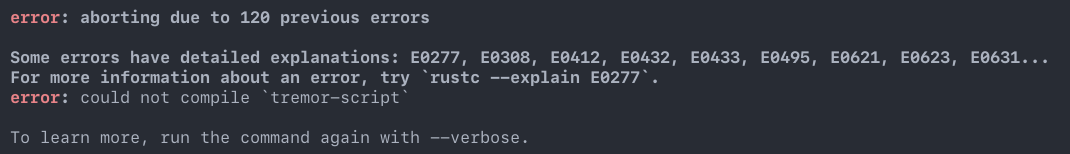
\includegraphics[width=\textwidth]{./Imagenes/errors.png}
    \caption{Al intentar evitar los tipos externos se produjeron más de 120
    errores de compilación.}%
    \label{fig:errors}
\end{figure}

\subsection{Encapsular el tipo externo}

Otra opción es crear un \emph{wrapper} para \code{halfbrown}, de la misma forma
que lo hace ya \abistable con otras librerías más conocidas. Este
encapsulamiento hace posible su uso desde el ABI de C de forma segura. Sin
embargo, estos ejemplos ya existentes son complejos~\cite{complexwrapper} y
difíciles de mantener, ya que tendrán que actualizarme con cada nueva versión de
\code{halfbrown}.

\begin{figure}
    \centering
    \begin{minted}{rust}
// Así funciona la programación asíncrona en Rust; la primera
// función es prácticamente equivalente a la segunda.
async fn example() -> String {
    read_file().await
}
fn example() -> impl Future<Output = String> {
    async {
        read_file().await
    }
}

// No pueden haber genéricos en FFI, por lo que ahora `Future`
// es un tipo concreto `FfiFuture` en vez de un trait. La
// conversión de `Future` a `FfiFuture` se puede realizar con
// `into_ffi`.
fn example() -> FfiFuture<String> {
    async move {
        read_file().await
    }
    .into_ffi()
}
// `FfiFuture<T>` implementa `Future<Output = T>`, por lo que
// su uso es el mismo.
async fn user() {
    example().await
}
    \end{minted}
    \caption{Interfaz modificada para la programación asíncrona en el sistema de
    plugins con la \crate \code{async_ffi}.}%
    \label{fig:async_ffi}
\end{figure}

\subsection{Reimplementar el tipo con el ABI de C desde cero}

Similar a la solución anterior, pero con incluso más costoso, dado que también
requeriría reimplementar la funcionalidad. Puede parecer indeseable, pero es la
mejor forma de asegurar un rendimiento máximo. Los tipos externos mencionados
son parte de optimizaciones; encapsularlos podría tener un impacto en su
rendimiento y hacerlos inútiles.

Si esta parte del proyecto es lo suficientemente importante y existen los
recursos, debería considerarse. De hecho, el mismo tipo \rust{Value} en Tremor
surgió por esta razón: ya existía \rust{simd_json::Value} de otra librería, pero
carecía de la suficiente flexibilidad y el equipo implementó uno personalizado.

\subsection{Simplificar el tipo para la interfaz}

Esta última opción resultó ser la más sencilla de implementar: crear una copia
de \rust{Value} cuyo único uso es para comunicarse entre runtime y plugins,
ilustrado en la Figura~\ref{fig:simplify}.

\begin{figure}
    \centering
    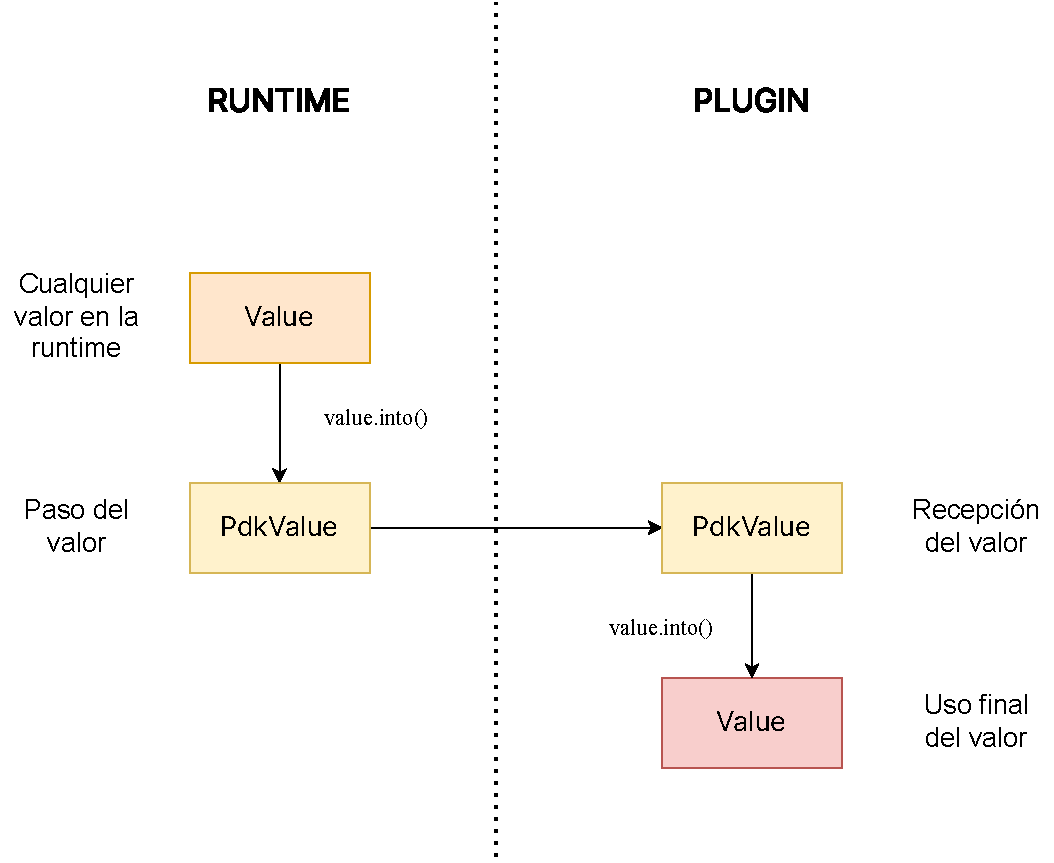
\includegraphics[width=10cm]{./Imagenes/simplify.pdf}
    \caption{Comunicación entre runtime y plugins en el PDK.}%
    \label{fig:simplify}
\end{figure}

Ya que es un tipo nuevo, no se romperá nada del código ya existente, y
únicamente hará falta cambiarlo donde se use la interfaz. Su implementación es
sencilla (notar el cambio de nombre a \rust{PdkValue}):

\begin{minted}{rust}
pub enum PdkValue {
    /// Valores estáticos (enteros, booleanos, etc)
    Static(StaticNode),
    /// Tipo para cadenas de caracteres
    String(String),
    /// Tipo para listas
    Array(Vec<Value>),
    /// Tipo para objetos (mapas clave-valor)
    Object(Box<HashMap<String, PdkValue>>),
    /// Tipo para datos binarios
    Bytes(Vec<u8>),
}
\end{minted}

No es necesario escribir métodos adicionales para el nuevo \rust{PdkValue}, solo
sus conversiones desde y hasta el tipo original, \rust{Value}. Esto sería
equivalente a, en vez de pasar un \rust{Vec<T>} al PDK, reemplzarlo con un
\rust{*const u8} para los datos y un \rust{u32} para la longitud. Simplemente
consiste en simplificar los tipos en la interfaz, y convertirlos de vuelta para
usar la funcionalidad completa.

El problema principal es que la conversión entre tipos es ahora $O(n)$ en vez de
$O(1)$, dado que es necesario iterar los datos en los objetos y vectores para la
conversión. Su uso sería el siguiente:

\begin{minted}{rust}
// Esta función es exportada por el plugin. Funcionará porque
// `PdkValue` está declarado con el ABI de C.
pub extern "C" fn plugin_funfuncue: PdkValue) {
    let value = Value::from(value);
    value.do_func()
}

// Esto se puede implementar en la runtime para facilitar su uso,
// convirtiendo al tipo original.
fn runtime_wrapper(value: Value) {
    plugin_func(value.into());
}
\end{minted}

Es la alternativa más sencilla, pero implica un coste de rendimiento; dos
conversiones implican iterar los datos dos veces. Tras mediciones posteriores,
se verificó que convertir los datos era un 5-10\% de la ejecución del programa.
Es menos de lo esperado, pero sigue sin ser suficiente para Tremor.

También tiene un coste de usabilidad; en comparación con tener un único
\rust{Value}, es necesario convertir los tipos y posiblemente crear encapsularlo
con una función de más alto nivel (\rust{runtime_wrapper}). Es una tarea
relativamente trivial, por lo que se podría automatizar con macros procedurales
en Rust, pero esto debería dejarse para el final del proyecto.

En conclusión, esta alternativa es la más fácil de implementar en el corto plazo
y por tanto la que mejor sigue \work. Se puede visualizar la diferencia de
rendimiento entre usar \rust{PdkValue} y reimplementar el tipo con C ``desde
cero'' --- hecho para la segunda versión --- en el Anexo~\ref{annex:benchmarks}.
